\subsection{Сценарий 1. Simple Speaker Listener}

Сходимость этого сценария становится возможной, когда \textit{говорун} сообщает правильные целевые ориентиры и \textit{слушатель} достигает их. В проведённых экспериментах агенты обучались с помощью алгоритмов MADDPG и DDPG.

\begin{figure}[ht!]
    \center
    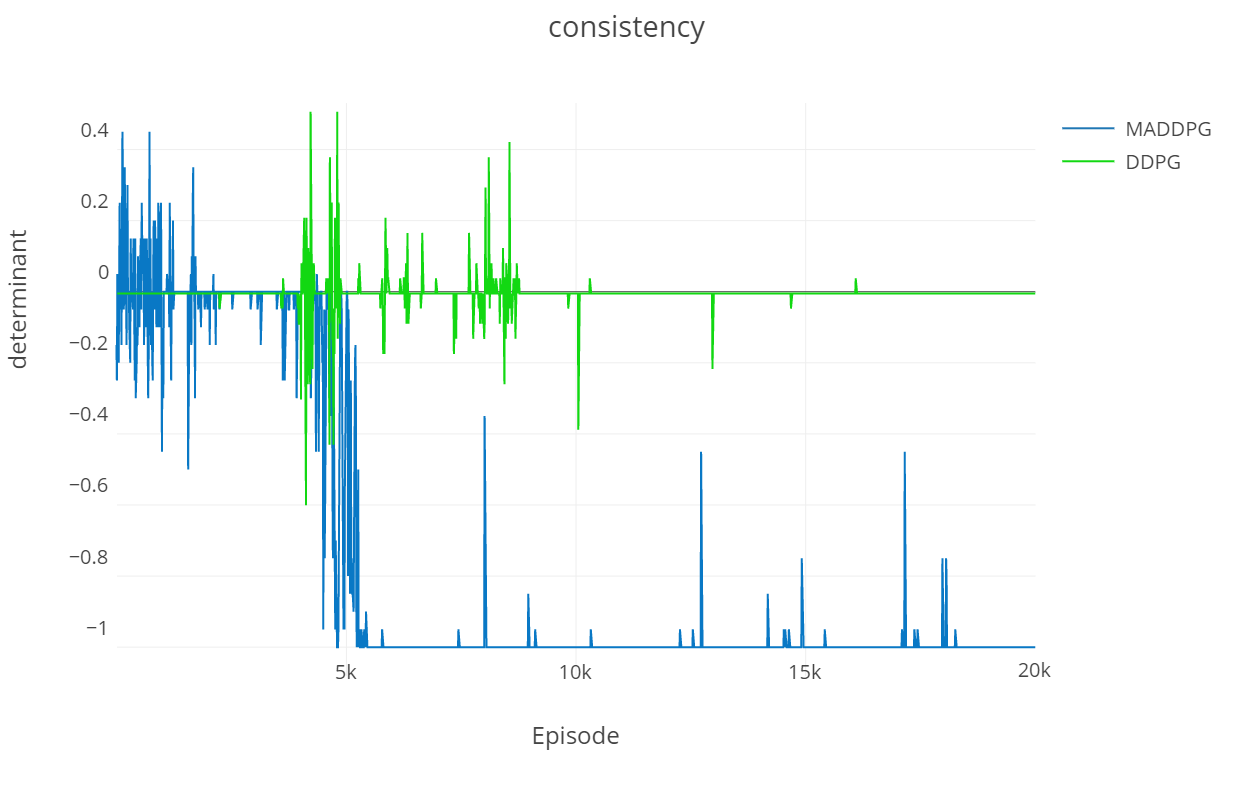
\includegraphics [scale=0.38] {my_folder/images/ch5/ssl-comm.png}
    \caption{График согласованности коммуникаций \textit{говоруна} в сценарии \textit{Simple Speaker Listener}}
    \label{fig:result-ssl-comm}
\end{figure}

Были построены графики согласованности коммуникаций и вознаграждений для двух агентов в сценарии \textit{Simple Speaker Listener}, которые представлены на \firef{fig:result-ssl-comm} и \firef{fig:result-ssl-rew}. На этих графиках синяя кривая~--- это результат обучения MADDPG, а зелёная~--- DDPG.

График на \firef{fig:result-ssl-comm} показывает сходимость консистентности действий общения для \textit{говоруна}, как описано в разделе \hyperref[exp-ssl]{Сценарии}. Этот график показывает, что сходится он только для MADDPG. Это указывает на то, что \textit{говорун}, обученный MADDPG, может постоянно интерпретировать ориентир в одной и той же кодировке, в то время как \textit{говорун}, обученный DDPG, не может поддерживать консистентное общение.

\begin{figure}[ht!]
    \center
    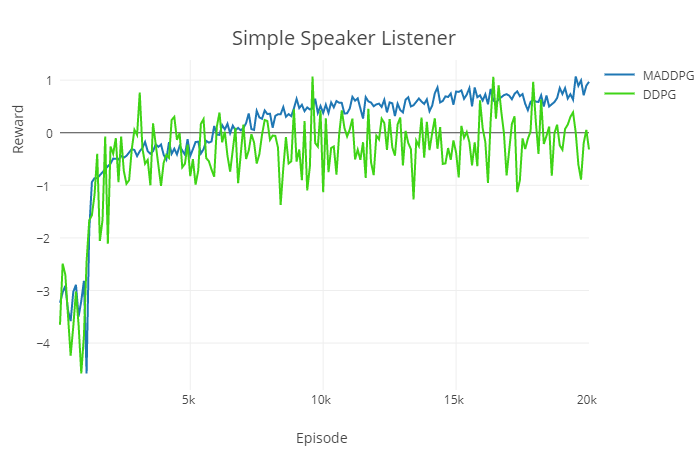
\includegraphics [scale=0.60] {my_folder/images/ch5/ssl-rew.png}
    \caption{График среднего вознаграждения для двух агентов в сценарии Simple Speaker Listener. Результаты обучения по алгоритму MADDPG и DDPG}
    \label{fig:result-ssl-rew}
\end{figure}

График на \firef{fig:result-ssl-rew} показывает среднее вознаграждение, которое агенты получили в конце каждого эпизода. Из этого графика видно, что вознаграждение, полученное агентами, обученными DDPG, ниже, чем агентами, обученными MADDPG.

\begin{figure}[ht!]
    \center
    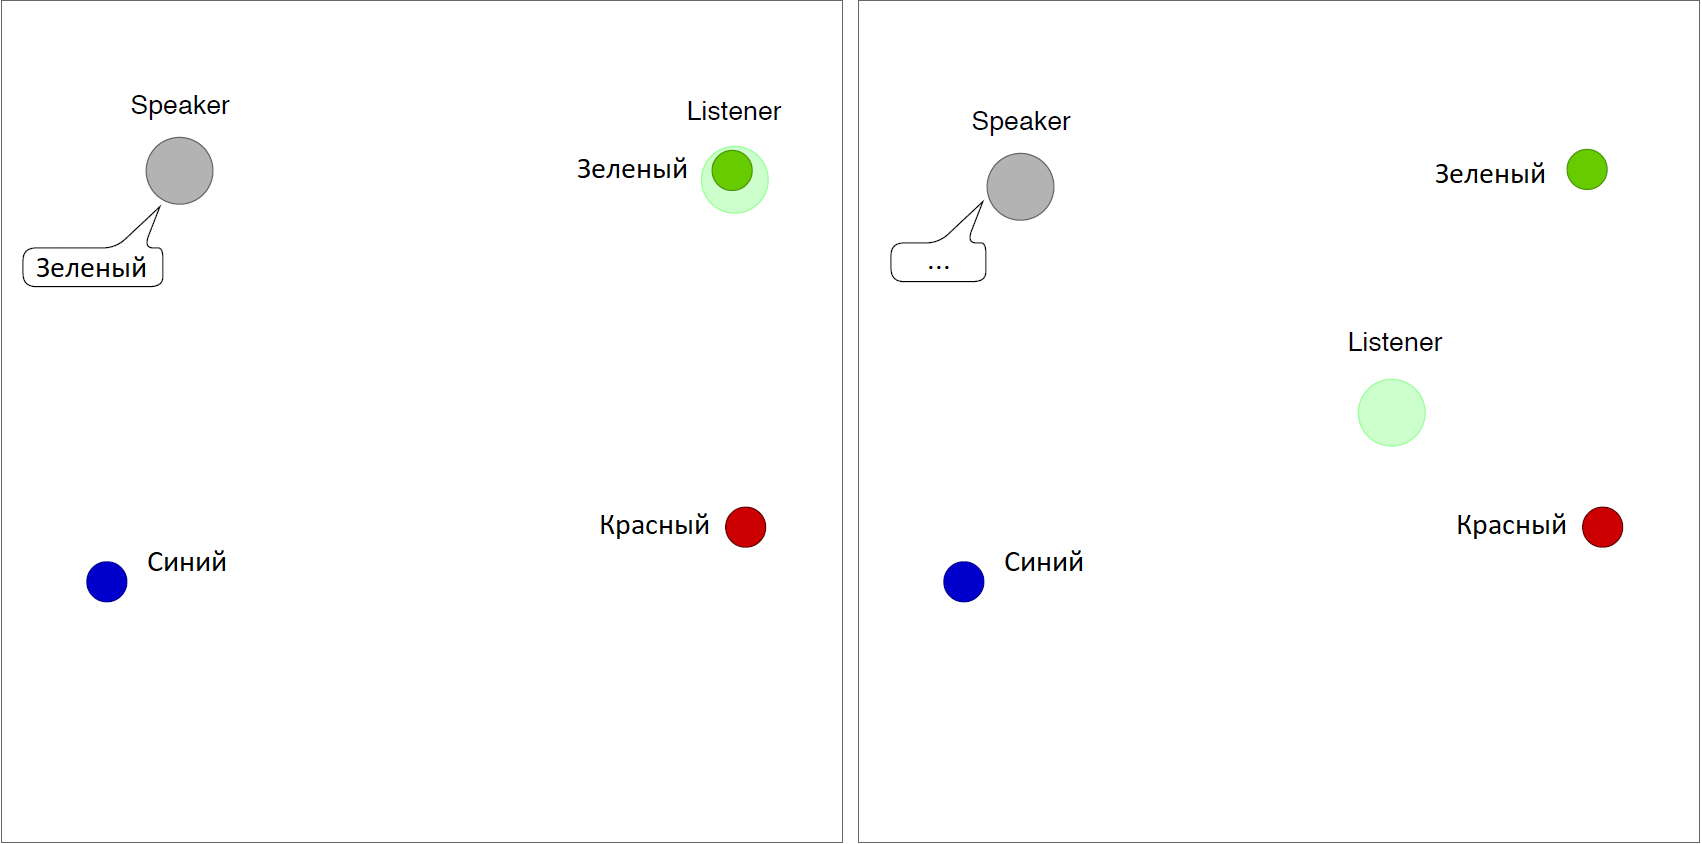
\includegraphics [scale=0.45] {my_folder/images/ch5/results-ssl-conv-non-conv.png}
    \caption{На левой стороне: \textit{говорун} произносит корректное высказывание, \textit{слушатель} перемещается к цели. Справа: коммуникационное действие отсутствует, и \textit{слушатель} застревает между тремя ориентирами (видимо, в попытке минимизировать расстояние до каждого из них)}
    \label{fig:result-conv-non-conv}
\end{figure}

Агенты, обученные DDPG, предпринимают действия, не имея полного наблюдения за состоянием окружающей среды и политикой других агентов. Они не в состоянии вычислить политику оптимального взаимодействия друг с другом.

На \firef{fig:result-conv-non-conv} показан скриншот при сходимости и отсутствии сходимости \textit{Simple Speaker Listener}.
